\subsection{Machine Learning for Quantum Error Mitigation}
\label{sec:liaoMachineMit}

\cite{liao_machine_2024}
% coherent vs incoherent errors
Machine learning can be used to directly mitigate errors as shown bi Liao et al \cite{liao_machine_2024}.
Training data is produced by running the same circuit on both a noisy backend and increasingly complex noise models of real quantum computers as provided by IBM through the \verb|qskit| python package \cite{javadi-abhari_quantum_2024}
Statistical models evaluated are ordinary least squares (OLS), random forest (RF), multi-layer perceptrons (MLP), and graph neural networks (GNN).
Zero noise extrapolation (ZNE) is used as a comparison state-of-the-art noise mitigation reference method.
Of the models evaluated, RF is found to perform the best with a mean error of 0.077 compared to the unmitigated mean error of 0.166 and ZNE with a mean error of 0.118.
A full comparison of tested models can be found in figure \ref{fig:liao_comparison}.

The data generation methods described here - increasingly noisy calculations on a simulated backend - can easily serve as a reference for generating our own training data.  % good here? no need to simulate exact noise sources?
As a key difference, our framework has the additional goal of identifying primary source(s) of noise in the quantum computer and use this information to employ an optimal mitigation method.

\begin{figure}[t]
    \centering
    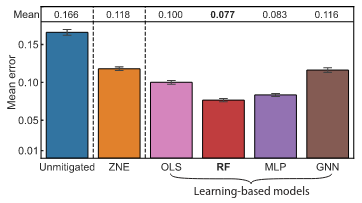
\includegraphics[width=0.5\linewidth]{figures/liao_comparison.png}
    \caption{Comparison of model errors from Liao et al. \cite{liao_machine_2024}}
    \label{fig:liao_comparison}
\end{figure}
